% Delphine 

  Nous avons pensé à étudier les contours grâce aux projections en X et en Y de l'image. 
L'idée est de faire apparaître les pics de pixel noir au niveau des contours. 

  Afin de retrouver algorithmiquement les positions des lignes verticales et horizontales qui définissent les carrés du \rubic{}, 
nous avons décidé de dériver les projections afin de déduire les positions en X et en Y de ces lignes. 

\subsubsection*{Principe de la méthode} 

  Cette méthode est basée sur l'étude de la dérivée. 
Elle suit les étapes suivantes : 
\begin{enumerate}
  \item Trouver les extremums. 

  L'étude du signe de la dérivée nous permet de localiser les extremums. 
En effet, leurs positions correspondent aux endroits où la dérivée change de signe, c'est à dire passe par zéro. 
Comme la dérivée a très peu de chance de valoir zéro, nous avons étudié le changement de signe de celle-ci. 

  Nous obtenons les positions de tous les extremums. 

  \item Trouver les minimums. 

  Les changements de signe dans le cas de minimum vont passer d'un signe positif à un négatif de la dérivée. 
Ainsi, nous avons récupéré sur l'ensemble des positions des extremums précédemment identifiés uniquement celles qui 
correspondent à la valeur 1 sur le vecteur caractéristique du signe de la dérivée. 

  Nous obtenons les positions de tous les minimums locaux. 

  \item Trouver le bon nombre de minimum en respectant une distance définie entre chacun de ces minimums. 
 
La méthode consiste à remplir une liste d'indices initialement vide avec les positions de minimum intelligemment choisies : 
  \begin{itemize}
    \item On récupère le minimum du vecteur en entrée dont l'indice correspond aux positions possibles, 
    \item Si la liste d'indices est vide, on l'ajoute; 
Sinon on calcule la distance minimale entre lui et les positions déjà contenues dans la liste d'indices 
et on la compare à celle qui définie la condition de distance voulue entre les minimums : 

  Si le distance calculée est supérieure, la position est ajoutée à la liste d'indices ; Sinon, non. 
    \item Afin que ce minimum ne soit plus considéré au cours des futures itérations, 
on modifie la valeur du vecteur à cette position tel qu'il prennent la valeur maximale de ce vecteur. 
  \end{itemize}
\end{enumerate}

  La signature de la fonction créée est la suivante : \\
\textit{function [indicePicMin]=detectionPicDerivee(VecteurEtudie, nbPic, largeurPic)}

\subsubsection*{Résultats obtenus par cette méthode}

     La figure~\ref{derivee_resultat_1} présente le résultat obtenu sur une image orientée et ayant subit un filtrage avec la méthode de la dérivée : 
 
 \begin{figure}[!h]
 \centering
 %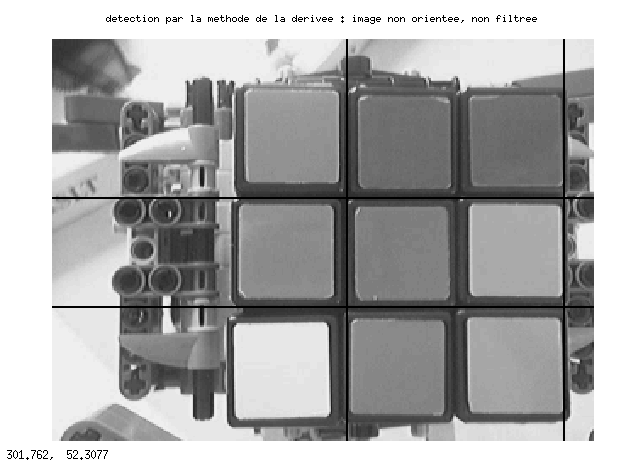
\includegraphics[width=0.45\linewidth]{Images/Derivee_img_traitement_1.png} 
 %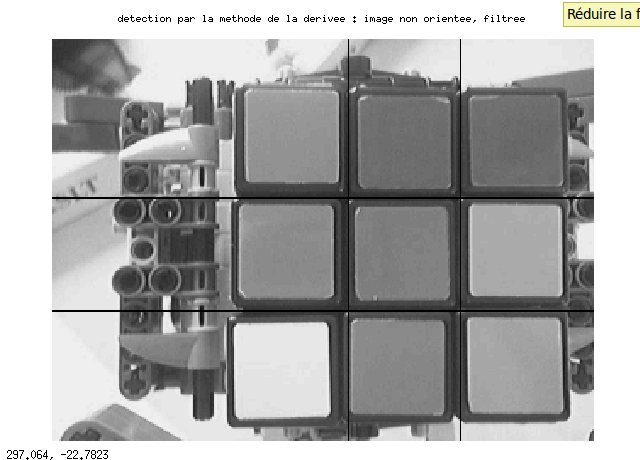
\includegraphics[width=0.45\linewidth]{Images/Derivee_img_traitement_2.png} \\
 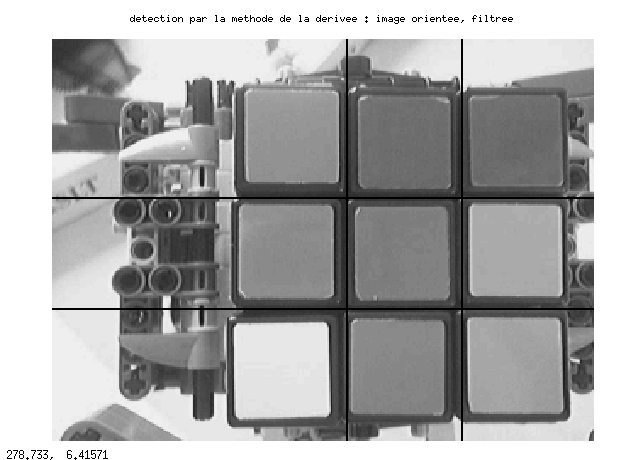
\includegraphics[width=0.9\linewidth]{Images/Derivee_img_traitement_3.png} 
 %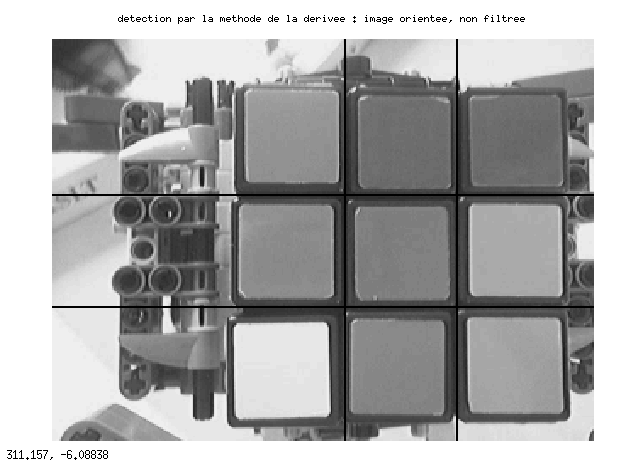
\includegraphics[width=0.45\linewidth]{Images/Derivee_img_traitement_4.png} 
 \caption{Résultat de la méthode dérivée} 
 \label{derivee_resultat_1}
 \end{figure}
